\documentclass{beamer}
\usepackage{graphicx}
\usetheme{Manhattan}
\title{From Individual\\to Population\\\Large (Challenges in Medical Visualization)}
\author{Maarten Inja, Chiel Kooijman}

\begin{document}
\begin{frame}
	\maketitle
\end{frame}

\begin{frame}
	Overall: Balancing realism, convention, and adding more information i.e.
	multi-subject (2.6, 3.10), time-variant (2.4), simulation (2.2, 3.5)\\
	
	\begin{itemize}
		\item 70s: CT and MRI $\rightarrow$ marching cubes\\
		\item Illustrative Rendering (2.5), Illustrative Visualization in
			Medicine (3.7)\\
		\item Integration of simulation (3.5) - also map uncertainty, Therapy
			planning, predictive simulation, diagnosis (2.2)\\

		\item People are used to interact with multi-touch (3.2)\\

		\item Interactive image Segmentation (Do we want to do this?) (3.3)\\

		\item Where do Topological methods (3.4) go? Do we address them?

		\item Mappings and Reformations (3.6) e.g. standardized way to
			represent part of the heart\\

		\item Hyper-realism (3.7, nice pictures) 3D cues help task performance,
			but effect of realism needs to be explored
	\end{itemize}
\end{frame}

\begin{frame}
	\frametitle{The 70s (2D)}
	\begin{center}
		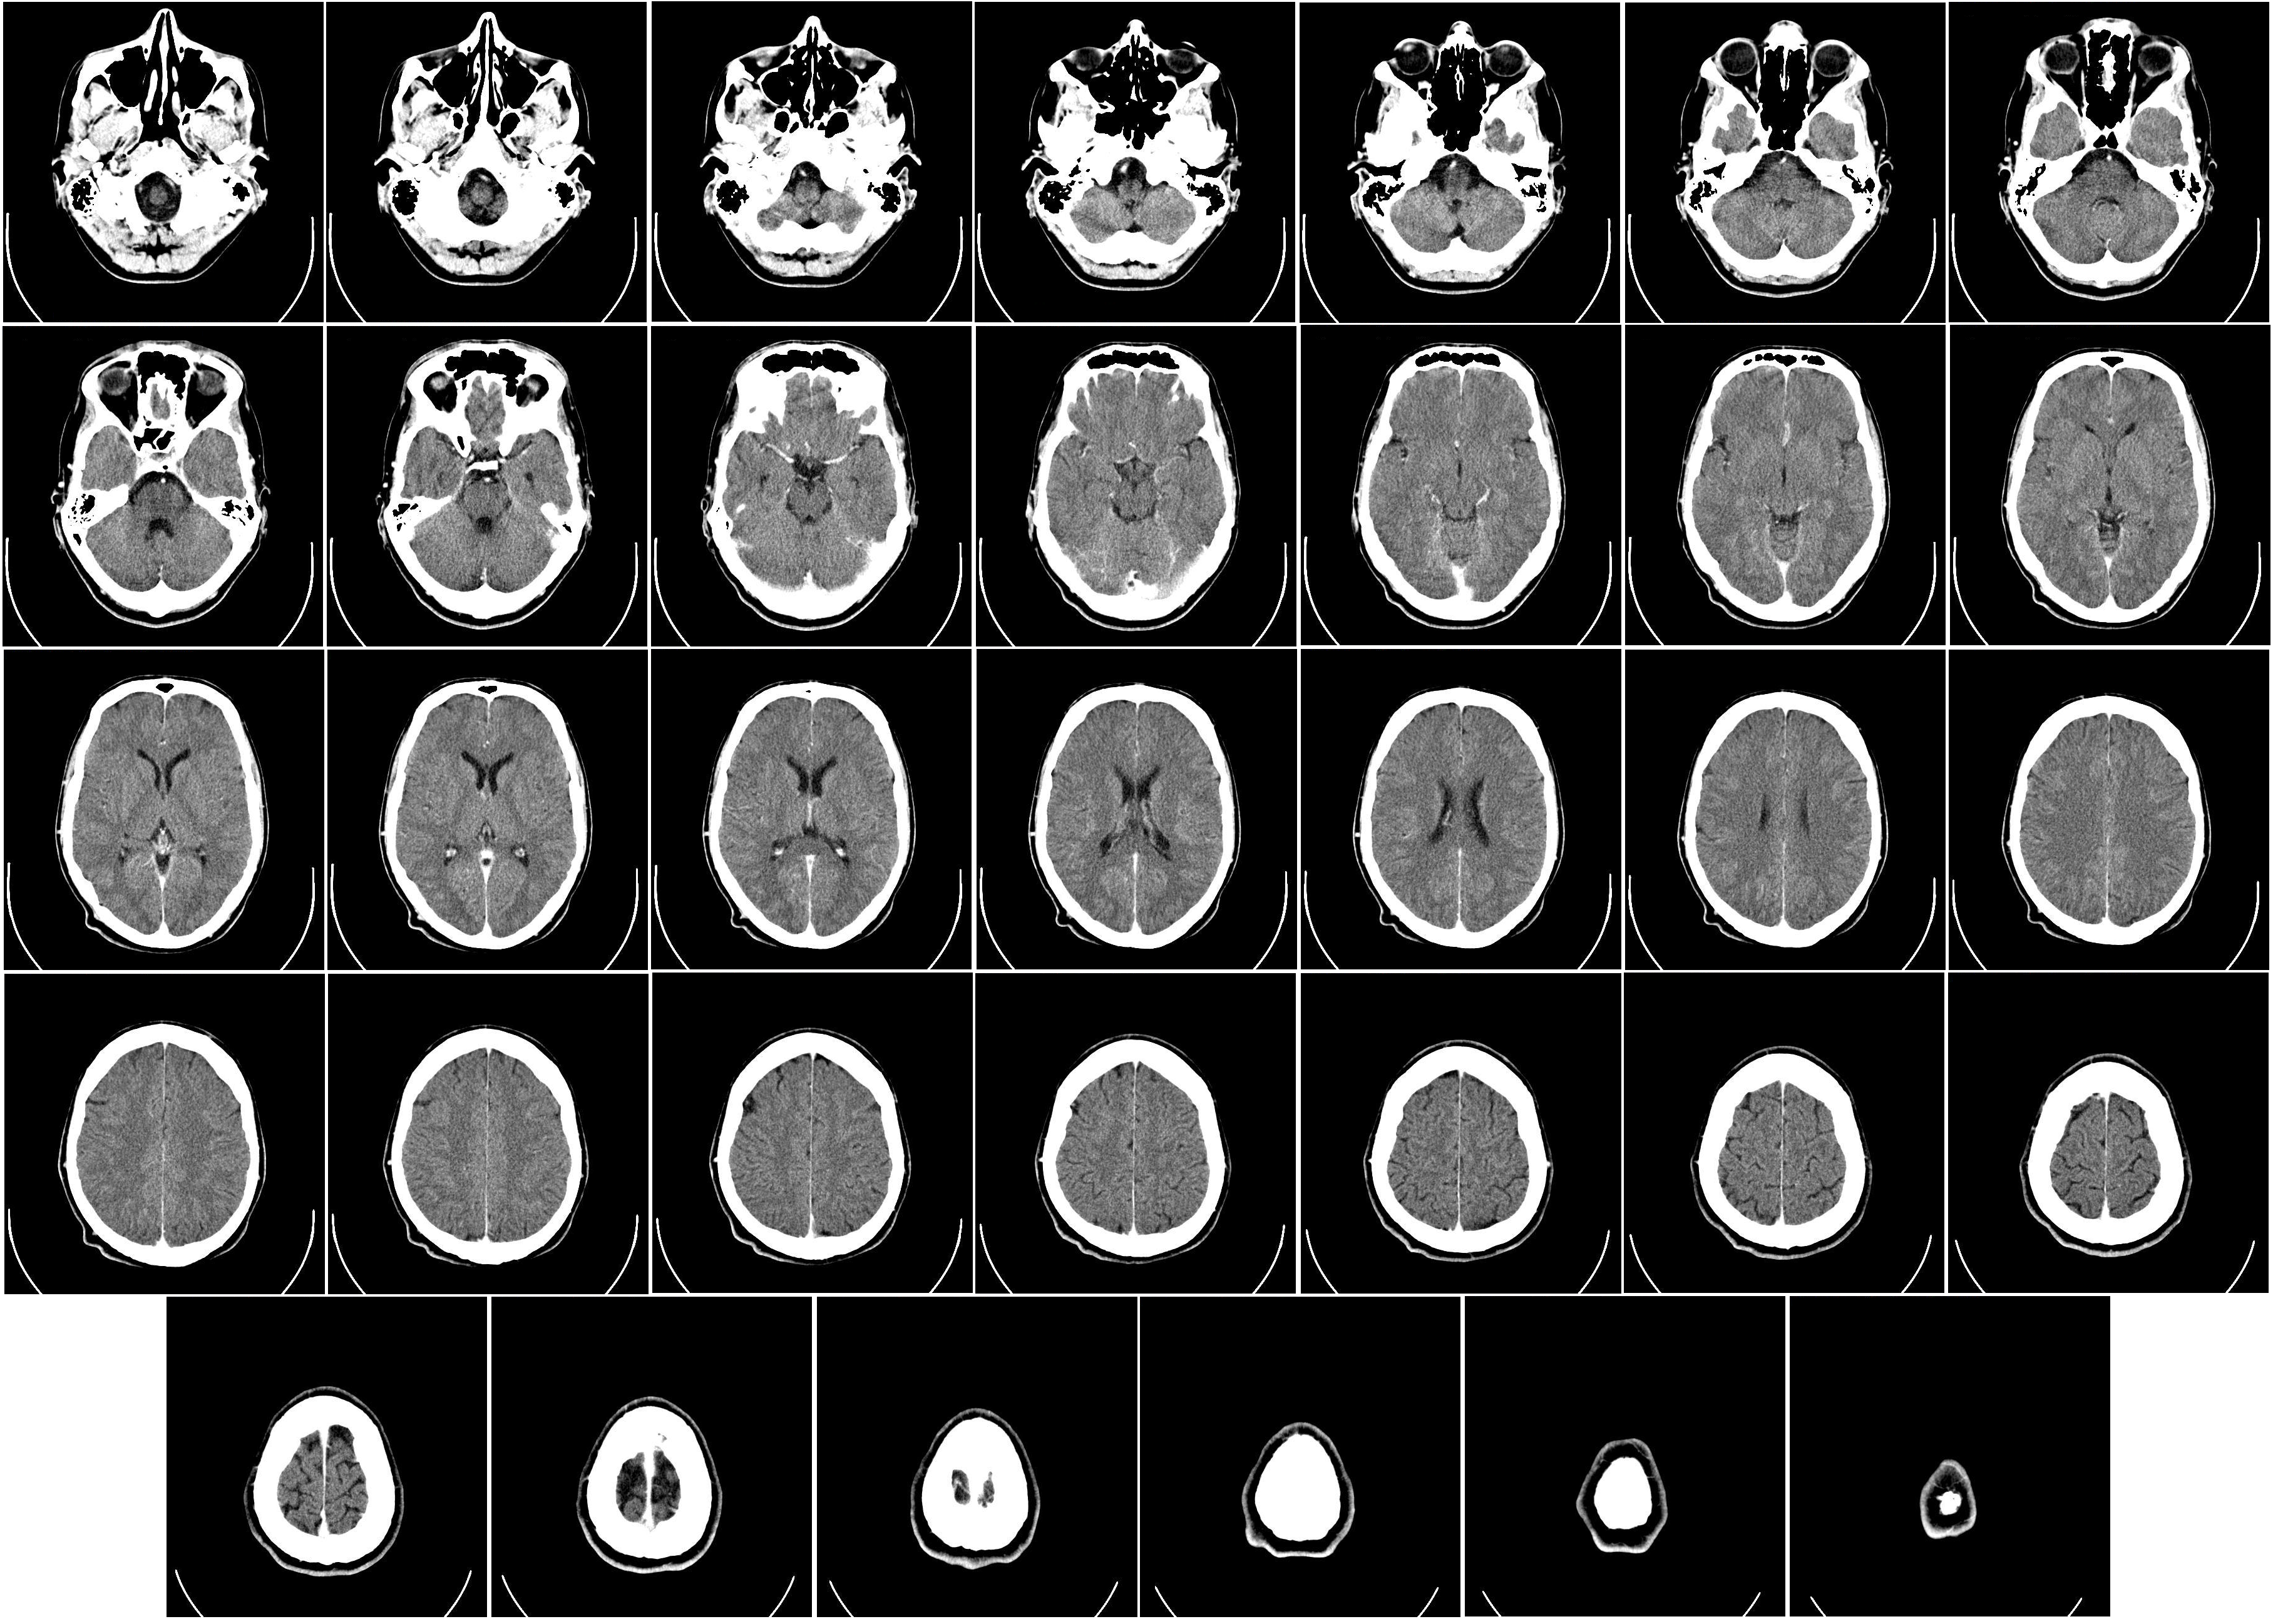
\includegraphics[width=.6\textwidth]{images/ct}
	\end{center}
	\begin{itemize}
		\item CT
		\item MRI
	\end{itemize}
\end{frame}

\begin{frame}
	\frametitle{The 80s (3D)}
	\begin{itemize}
		\item Marching Cubes (CT)
	\end{itemize}
	\begin{center}
		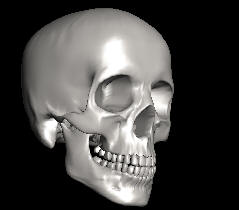
\includegraphics[width=.4\textwidth,height=.4\textheight]{images/marching}
	\end{center}
\end{frame}

\begin{frame}
	\frametitle{More dimensions}
	Higher dimensional data due to:
	\begin{itemize}
		\item Time-variance
		\item Multi-field (DTI, tensors)
		\item Simulation
		\item Multiple sources
			\begin{itemize}
				\item Multi-subject
				\item Multi-modal
			\end{itemize}
	\end{itemize}
\end{frame}

\begin{frame}
	\frametitle{More dimensions}
	\textbf{Solutions:}\\
	Add interactivity:
	\begin{itemize}
		\item Multi-touch devices allow for more flexibility
	\end{itemize}
	Improved visualizations:\\
	\begin{itemize}
		\item Topological methods
		\item Illustrative visualizations
	\end{itemize}
	versus
	\begin{itemize}
		\item Hyper-realism
	\end{itemize}
\end{frame}

\begin{frame}
	Mappings:
	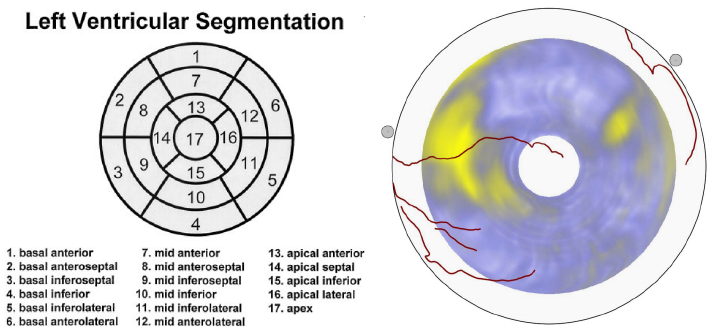
\includegraphics[width=\textwidth]{images/heart}
\end{frame}

\begin{frame}
	Illustrative (Zachow et al. 2009):
	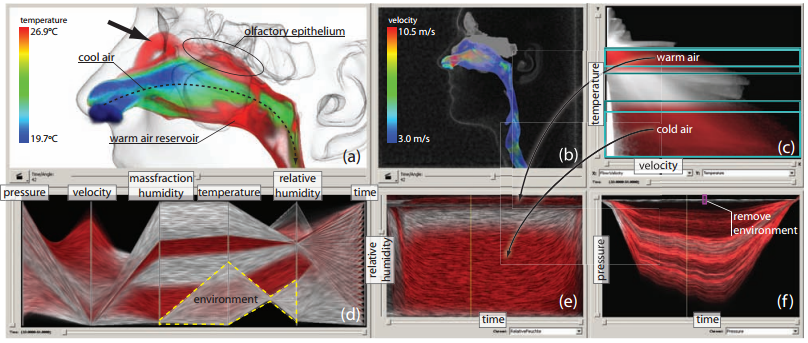
\includegraphics[width=\textwidth]{images/nose}
\end{frame}

\begin{frame}
	Illustrative - colon unfolding (Tietjen et al. 2005):
	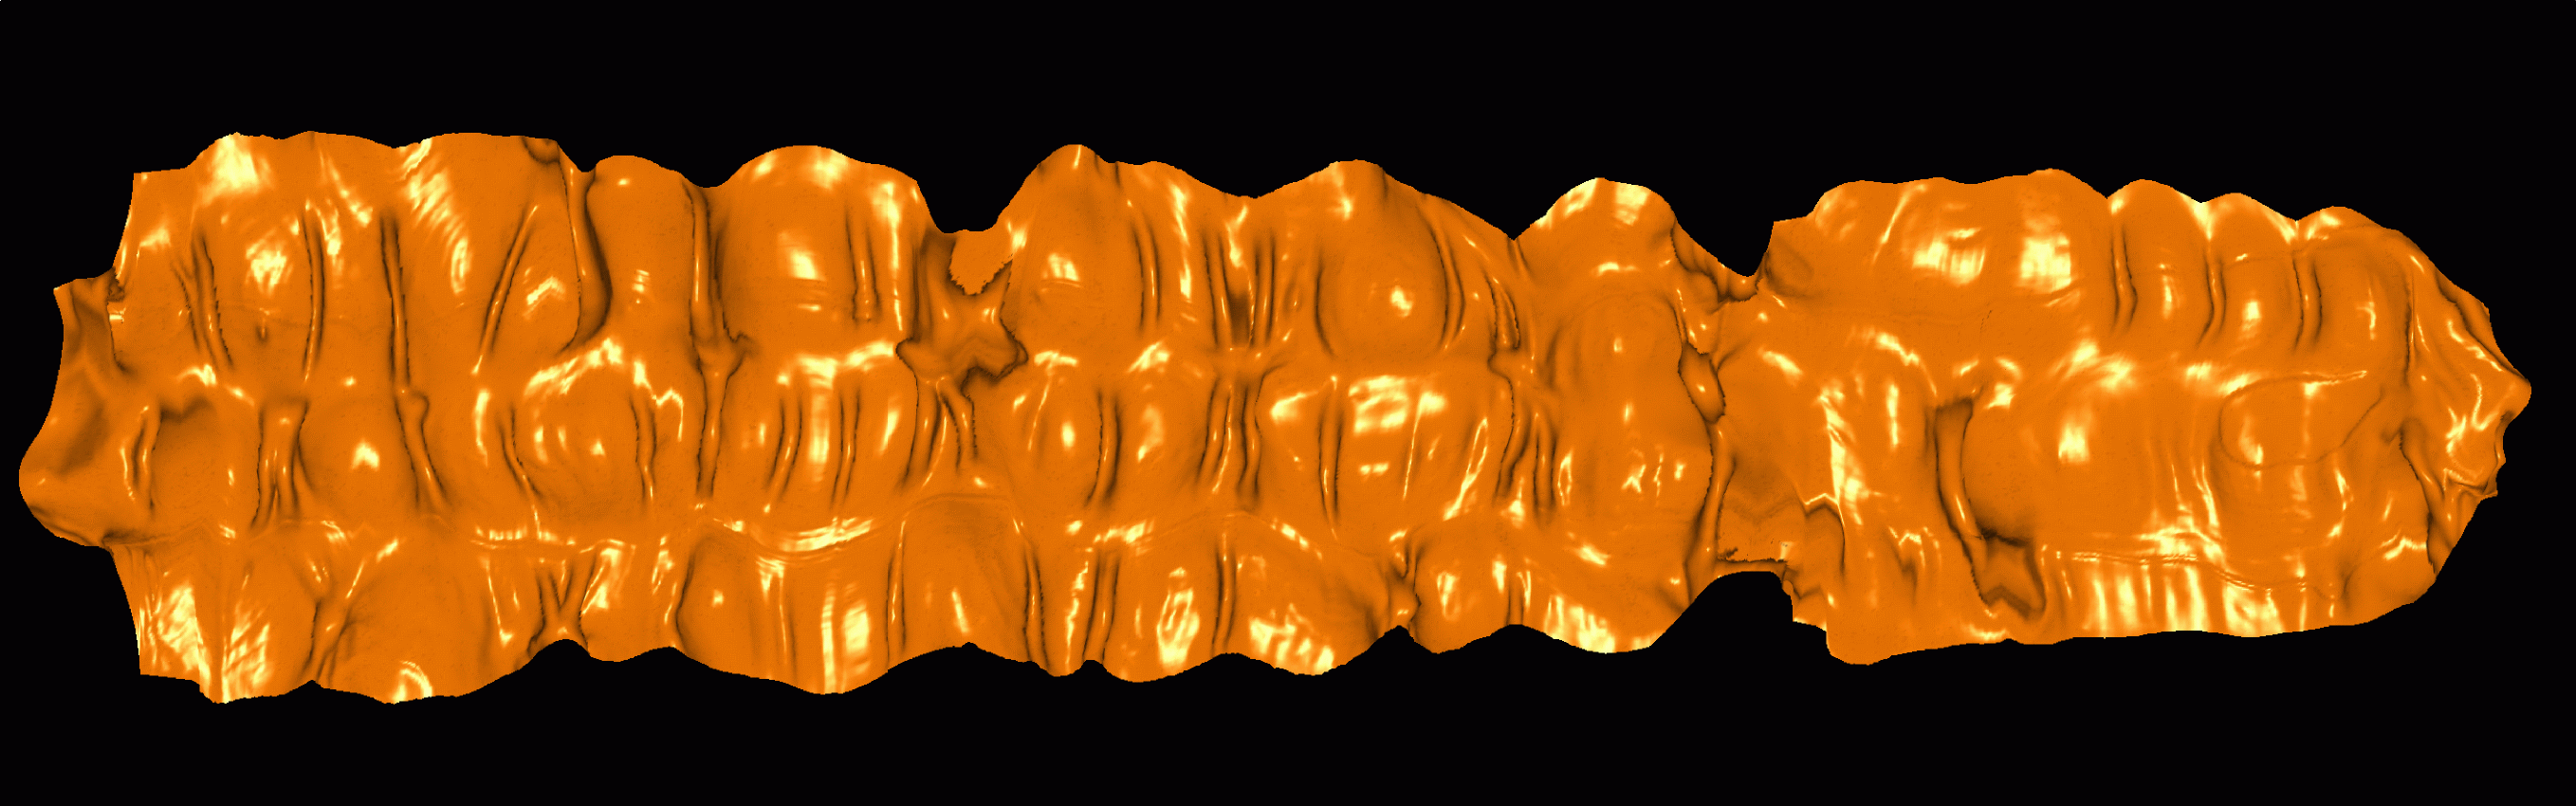
\includegraphics[width=\textwidth]{images/colon}
\end{frame}

\begin{frame}
	DTI (2.3):
	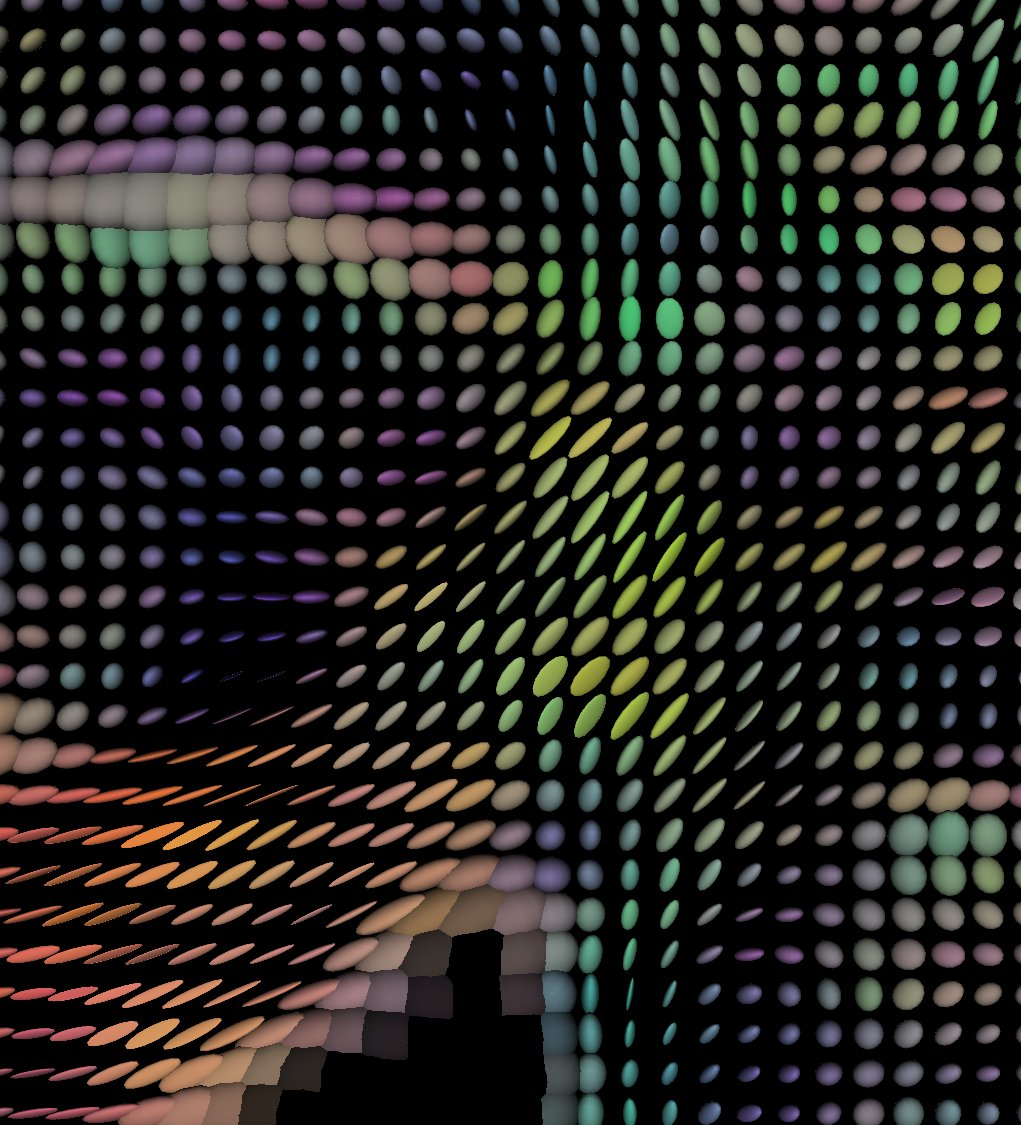
\includegraphics[width=\textwidth]{images/dti}
\end{frame}

\begin{frame}
	DTI (2.3):
	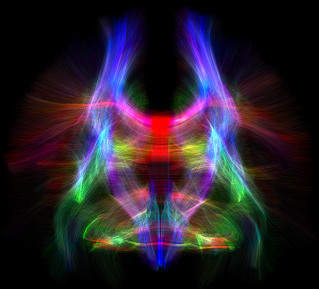
\includegraphics[width=\textwidth]{images/tractography}
\end{frame}

\begin{frame}
	Realism:
	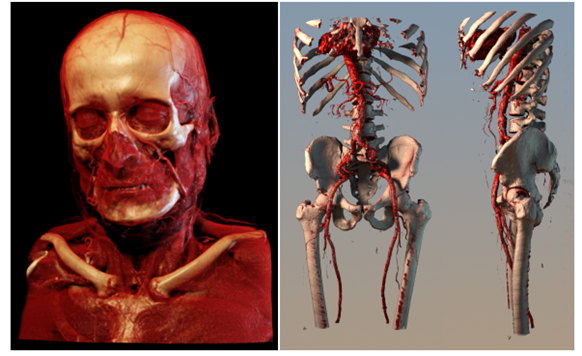
\includegraphics[width=\textwidth]{images/medical_visualisation}
\end{frame}

\begin{frame}
	Realism:
	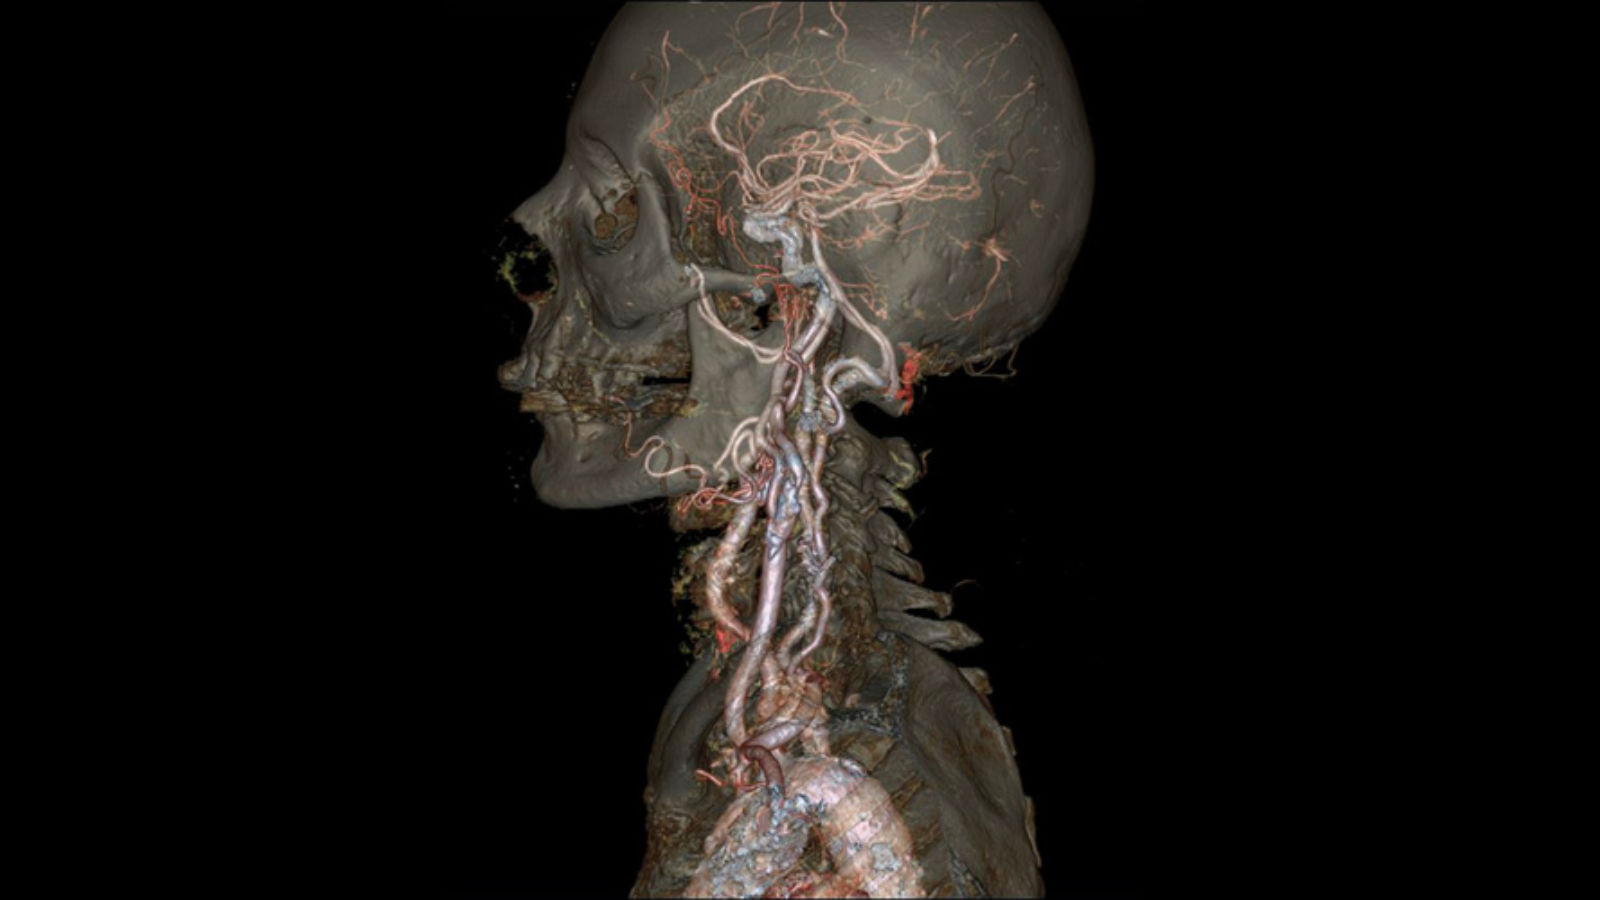
\includegraphics[width=\textwidth]{images/realistic_transparent}
\end{frame}
\end{document}
% vim: spell
